
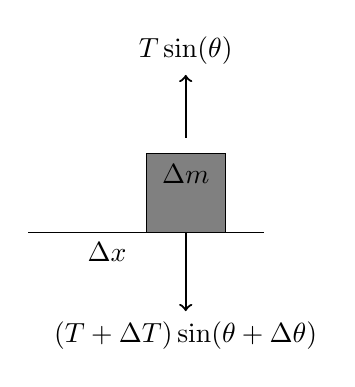
\begin{tikzpicture}
    % Draw the string element
    \draw (0,0) -- (3,0);
    
    % Draw the square block
    \draw[fill=gray] (1.5,0) rectangle (2.5,1);
    
    % Label the length and mass
    \node[below] at (1,0) {\( \Delta x \)};
    \node[above] at (2,0.5) {\( \Delta m \)};
    
    % Add the upward tension force arrow
    \draw[->, thick] (2,1.2) -- (2,2) node[above] {\( T \sin(\theta) \)};
    
    % Add downward forces on the block
    \draw[->, thick, black] (2,0) -- (2,-1) node[below] {\(( T+\Delta T) \sin(\theta + \Delta \theta) \)};
    
\end{tikzpicture}


